%\documentclass[handout]{beamer}
\documentclass{beamer}

% Customize slide appearance
\mode<presentation>
{
  \usetheme{default}
%  \setbeamercovered{transparent}
}

\usepackage[english]{babel}
\usepackage{times}
\usepackage{threeparttable}
\usepackage{tabularx}
\usepackage{booktabs}
\usepackage{pgfpages}
\usepackage{latexsym,amsmath,amssymb,textcomp,eurosym,dcolumn,booktabs}
\usepackage{color}
\usepackage{colortbl}
\usepackage{graphicx}
\usepackage{amsthm}

\definecolor{darkblue}{rgb}{0.1,0,0.55} \definecolor{darkgreen}{rgb}{0,0.7,0}
\definecolor{important}{rgb}{0.9,0.1,0.1} %
\definecolor{hidden}{rgb}{0.8,0.8,0.8}
\definecolor{darkgreen}{rgb}{0,0.7,0}

\usenavigationsymbolstemplate{}
\setbeamertemplate{footline}
    {\begin{beamercolorbox}[sep=1ex]{author in head/foot}
      \hfill\llap{\insertframenumber}%
      \end{beamercolorbox}%
      }


%\pgfpagesuselayout{4 on 1}



\AtBeginSection[]
{
  \begin{frame}
  \frametitle{Outline}
  \large{\tableofcontents[currentsection,hideothersubsections]}
  \end{frame}
}


%\usepackage{amstext}

\begin{document}

\begin{frame}

\bigskip

\center{{\Large \textcolor{darkblue}{Seeing is Believing: \\ Identity, Inequality, and the Impact of Television on the Hispanic Achievement Gap}} \medskip}

\bigskip


\center{\textbf{Andrew Kao} \\ \textit{Harvard}}

\bigskip \bigskip

\center{AEFP --- March 2022}

\end{frame}


%%%%% MOTIVATION %%%%%%

%% Spanish achievement gap
\begin{frame}
\frametitle{Motivation (I): the Hispanic achievement gap is large}
\centering
        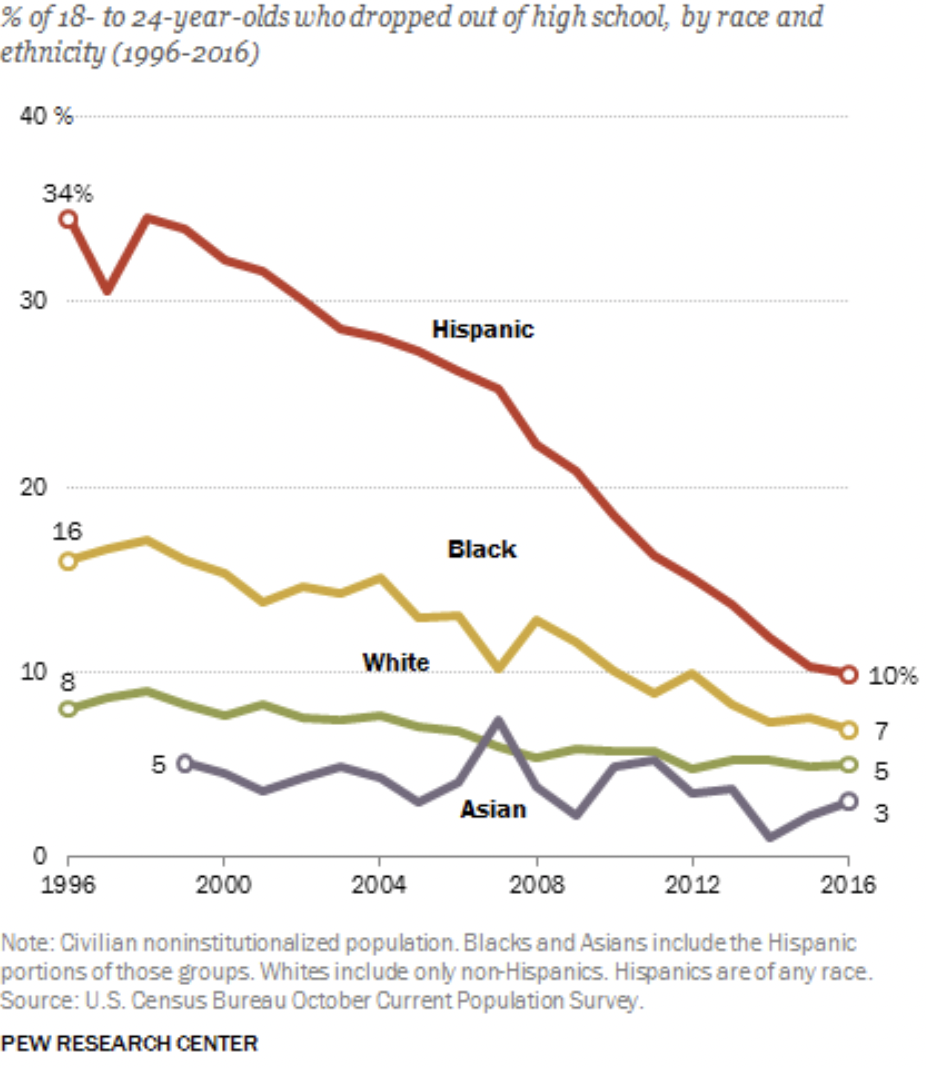
\includegraphics[width=.6\textwidth]{figs/hispanic_dropout.png}\\
\end{frame}

%% SLTV
\begin{frame}
\frametitle{Motivation (II): Americans \textit{really} love TV}
\vspace{1.5pt}
\centering
        
\includegraphics[width=\textwidth]{figs/tv_time1}
        \vspace{-3em}
\begin{flushright}
                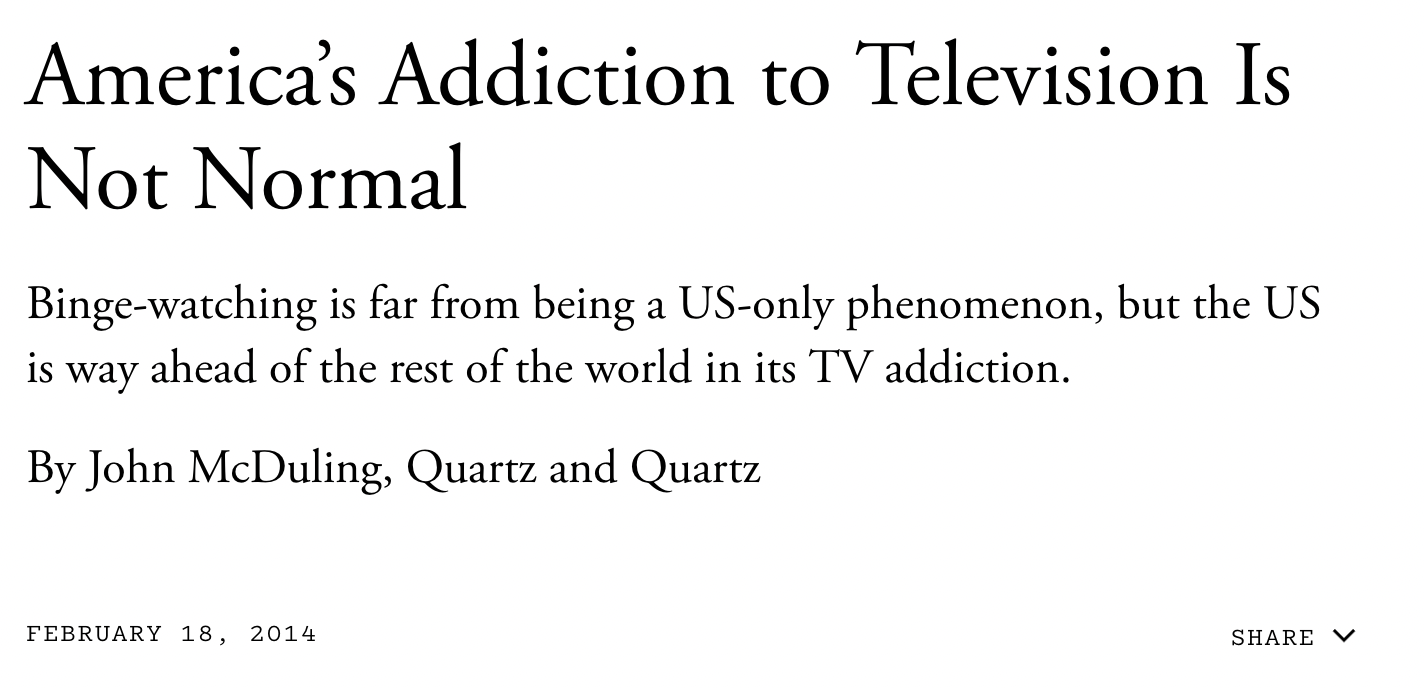
\includegraphics[width=.8\textwidth]{figs/tv_time4}
\end{flushright}
\vspace{-4em}
        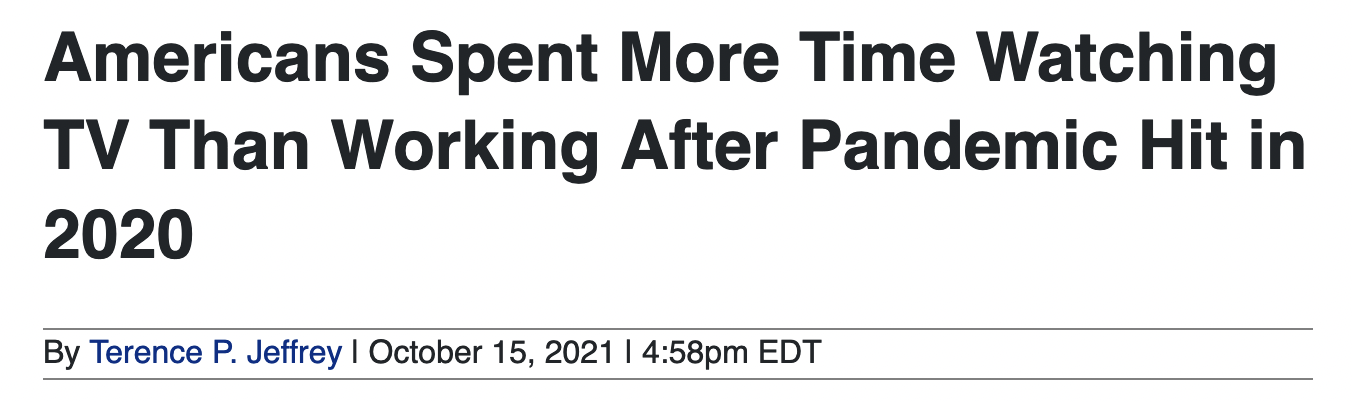
\includegraphics[width=\textwidth]{figs/tv_time2}\\
\end{frame}



%% Overall
\begin{frame}



\huge {\color{darkblue} How does Spanish Language TV affect Hispanic educational outcomes?}

\end{frame}


%%%%% PROJECT OVERVIEW %%%%%%
\begin{frame}
\frametitle{This project:}

Show that SLTV reduces the Hispanic achievement gap in public schools:
\vspace{1.5em}
\begin{itemize}
  \setlength\itemsep{1.5em}

\item Identification: difference-in-discontinuities design
\item Gap vs. whites and Asians in SAT/ACTs taken, calculus courses taken, AP exams passed, etc. \textbf{shrinks} with SLTV
\item However, the gap vs. whites and Asians \textbf{rises} when looking at English proficiency
\end{itemize}

\end{frame}

\begin{frame}
\frametitle{How to reconcile this?}


\pause 
Propose an \textbf{identity} mechanism. Four strands of evidence:
\vspace{1.5em}
\begin{enumerate}
  \setlength\itemsep{1.5em}
\item More bullying on the basis of ethnicity (but not gender)

\item Hispanics perform better where SLTV focuses more on Hispanic identity (but not on education)

\item Hispanics with SLTV visit Hispanic branded establishments more (but not Brazilian branded ones)

\item Counties with SLTV are more socially connected to LatAm
\end{enumerate}

\end{frame}



%%% COVERAGE MAP %%%
\begin{frame}
\frametitle{Coverage Map for TV Station WUVC-DT}
\centering
        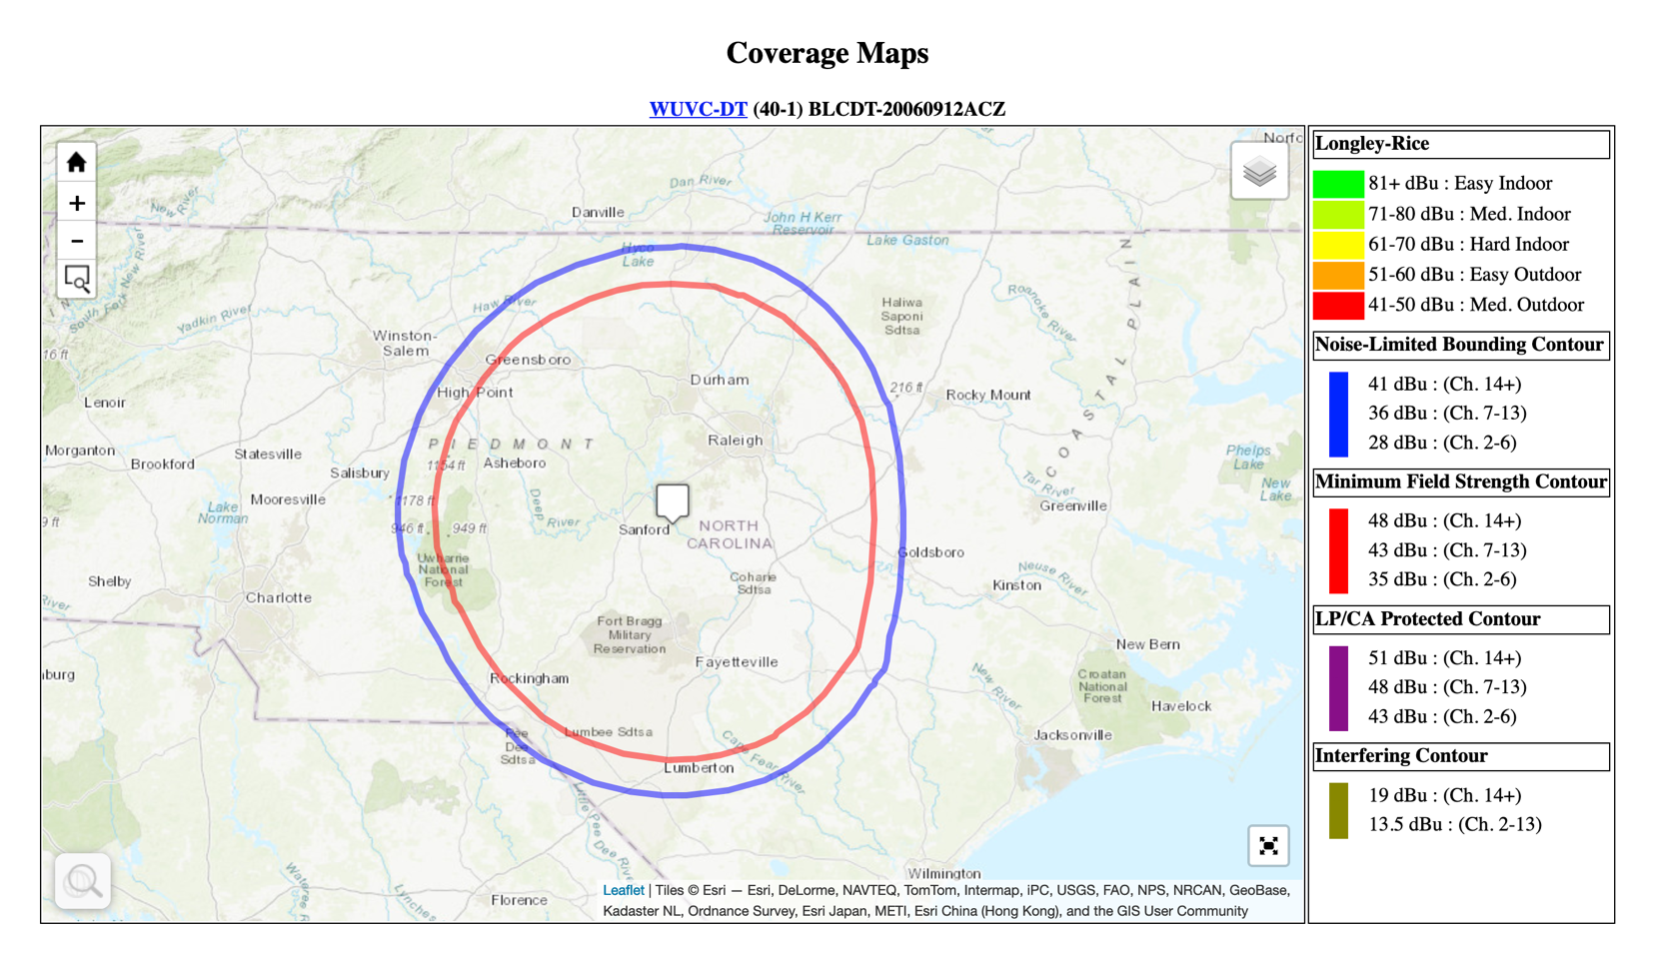
\includegraphics[width=1\textwidth]{../../analysis/Output/img/ContourExample.png}\\
\end{frame}

%%% EMPIRICAL STRATEGY %%%
\begin{frame}
\frametitle{Empirical Strategy}


\begin{itemize}
  \setlength\itemsep{1.5em}
\item Construct spatial RD arising from FCC TV signal regulation \textit{(OET Bulletin 69)}
\begin{itemize}
\item TV stations protected from interference only within certain coverage contour areas. Keep observations within 100 KM of the contour boundary
\item Follow Velez \& Newman (2019), expand from 2 counties to entire US
\item Spanish Language TV: Isolate causal effect on SLTV on Hispanic communities
\end{itemize}

\pause
\item Compare against outcomes among Asians
\begin{itemize}
\item Less likely to identify as Hispanic (or watch SLTV)
\item Combine RD with Asian `control' for difference in discontinuities
\end{itemize}

\end{itemize}

\end{frame}

%%% SPECIFICATIONS %%%
\begin{frame}
\frametitle{Empirical Specification}

\[ y_{i,j} =  \beta \mathbb{I}[InsideContour_{i,j}] \times \mathbb{I}[Hispanic_{i,j}] + \gamma_k + \delta  X_i + \epsilon_{i,j} \]

\vspace{5pt}

where $y_{i,j}$ is an outcome for observation $i$ (which may be an individual, school, or establishment) under demographic category $j \in \{$Hispanic, not Hispanic$\}$, $\gamma_k$ is fixed effect for school district $k$, and $X$ is a vector of controls for the observation. 


\end{frame}

%%% COUNTRY MAP %%%
\begin{frame}
\frametitle{SLTV coverage and public schools}
\centering
        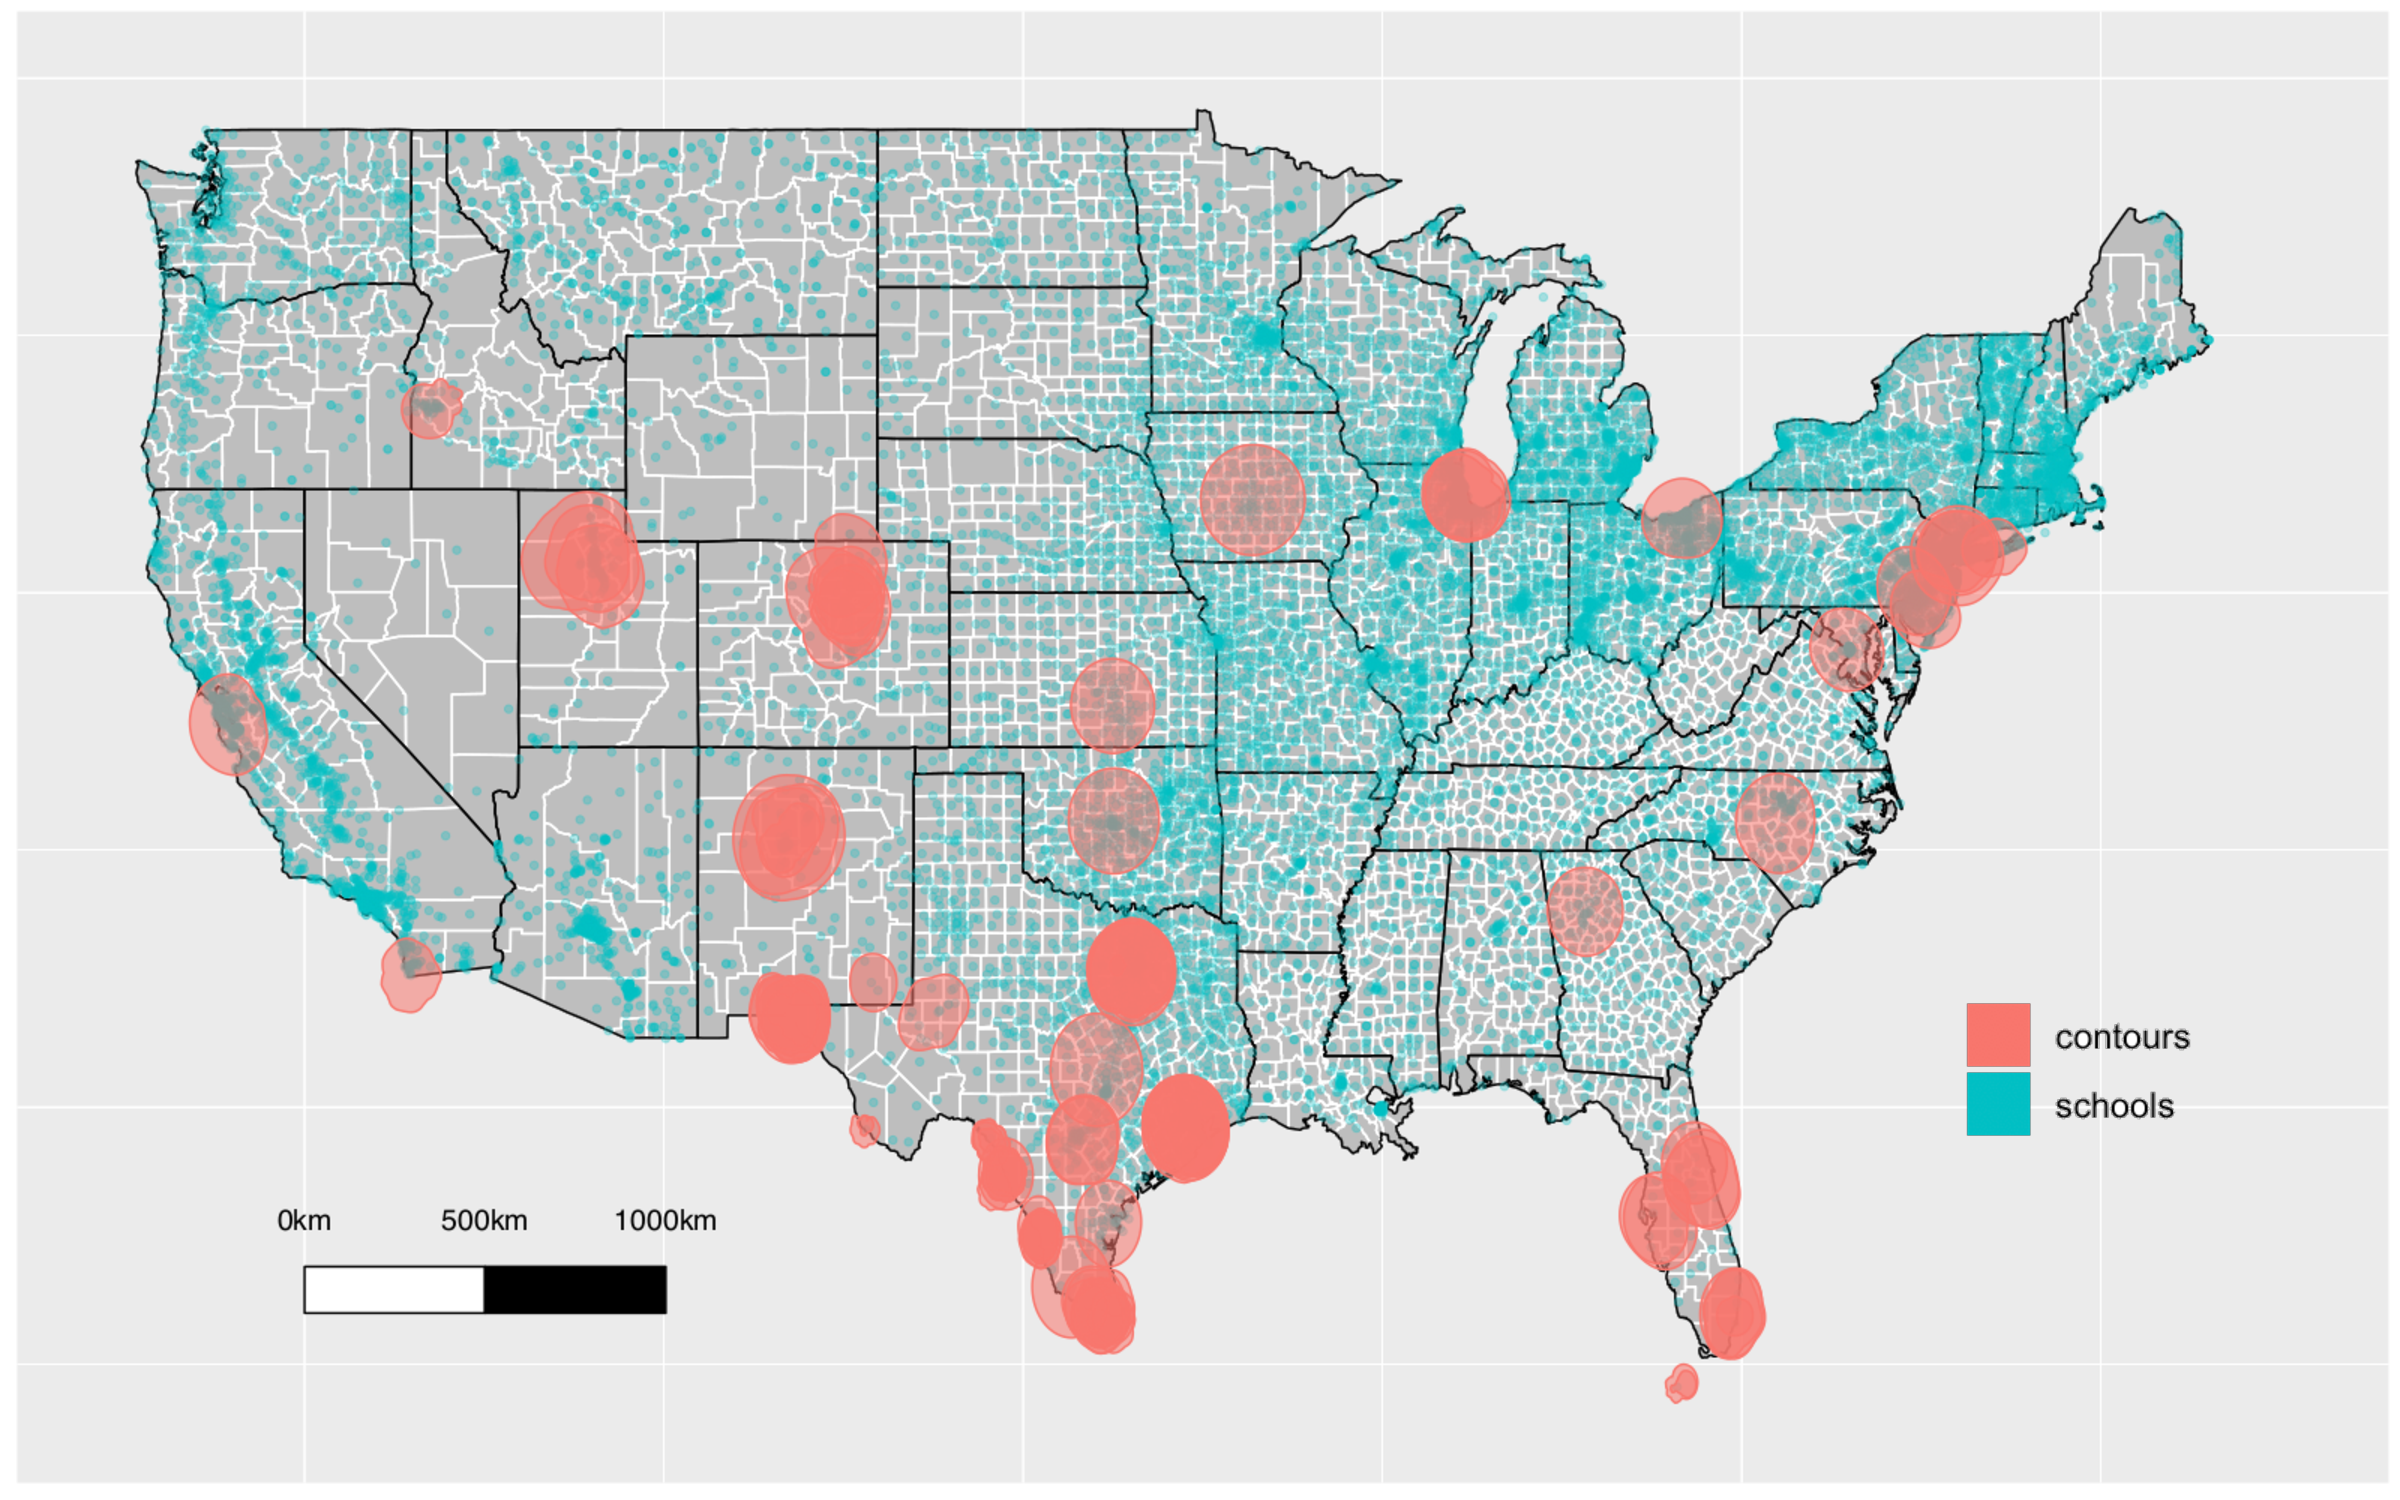
\includegraphics[width=1\textwidth]{../../analysis/Output/img/Schools_pretty2.pdf}\\
\end{frame}


%%% DATA %%%

\begin{frame}
\frametitle{Data}


\begin{itemize}
\item Instrument:
\begin{itemize}
\item Identify 100 Spanish Language TV stations across the US from \textbf{TMS}
\item Station contours and other station data from the \textbf{FCC}
\end{itemize}

\item \textbf{American Time Use Survey} over last 15 years:
\begin{itemize}
\item 210,000 person-year observations
\item Average person watches 170 minutes of TV per day
\end{itemize}

\item Department of Education's \textbf{Civil Rights Data Collection} in 2015:
\begin{itemize}
\item 48,000 public schools in sample (unit of observation)
\item Data on academic outcomes (SAT/ACTs taken, AP exams passed, etc.) \& other school data
\end{itemize}

\item Other measures of identity:
\begin{itemize}
\item TV transcript data from \textbf{archive.org}
\item Foot-traffic data from \textbf{Safegraph}
\item Social connectedness data from \textbf{Facebook}
\end{itemize}

%\item Demographic information at county/census block group level from ACS
\end{itemize}

\end{frame}



%%%% FIRST STAGE %%%%%

\begin{frame}
\frametitle{TV Viewership across the SLTV Boundary} \label{atus_time}

\begin{center}
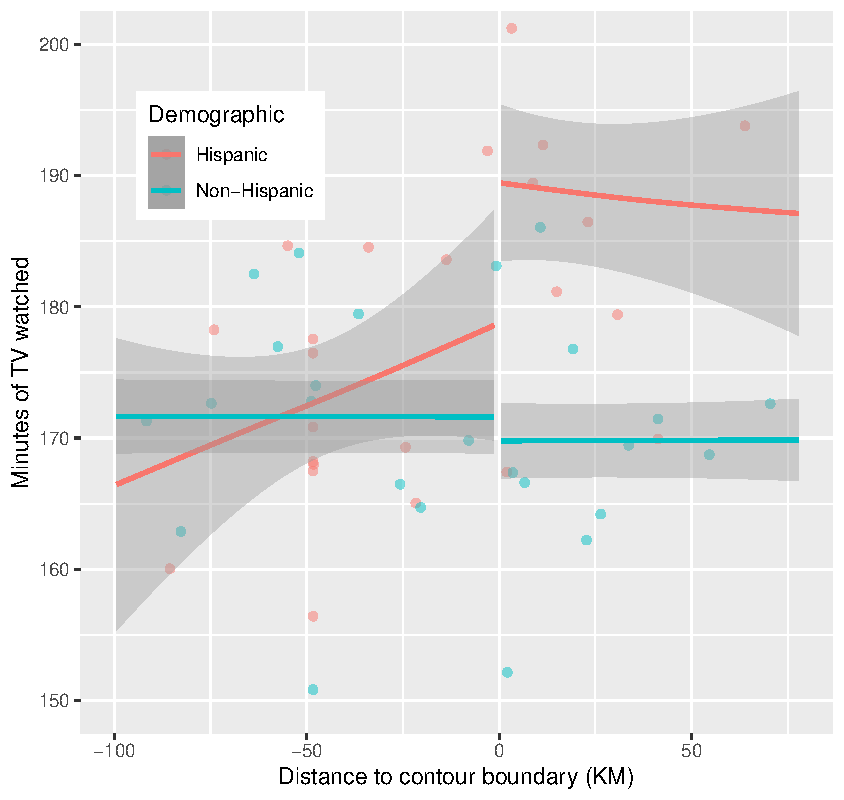
\includegraphics[width=.75\textwidth]{../../analysis/Output/graphs/atus2.pdf}
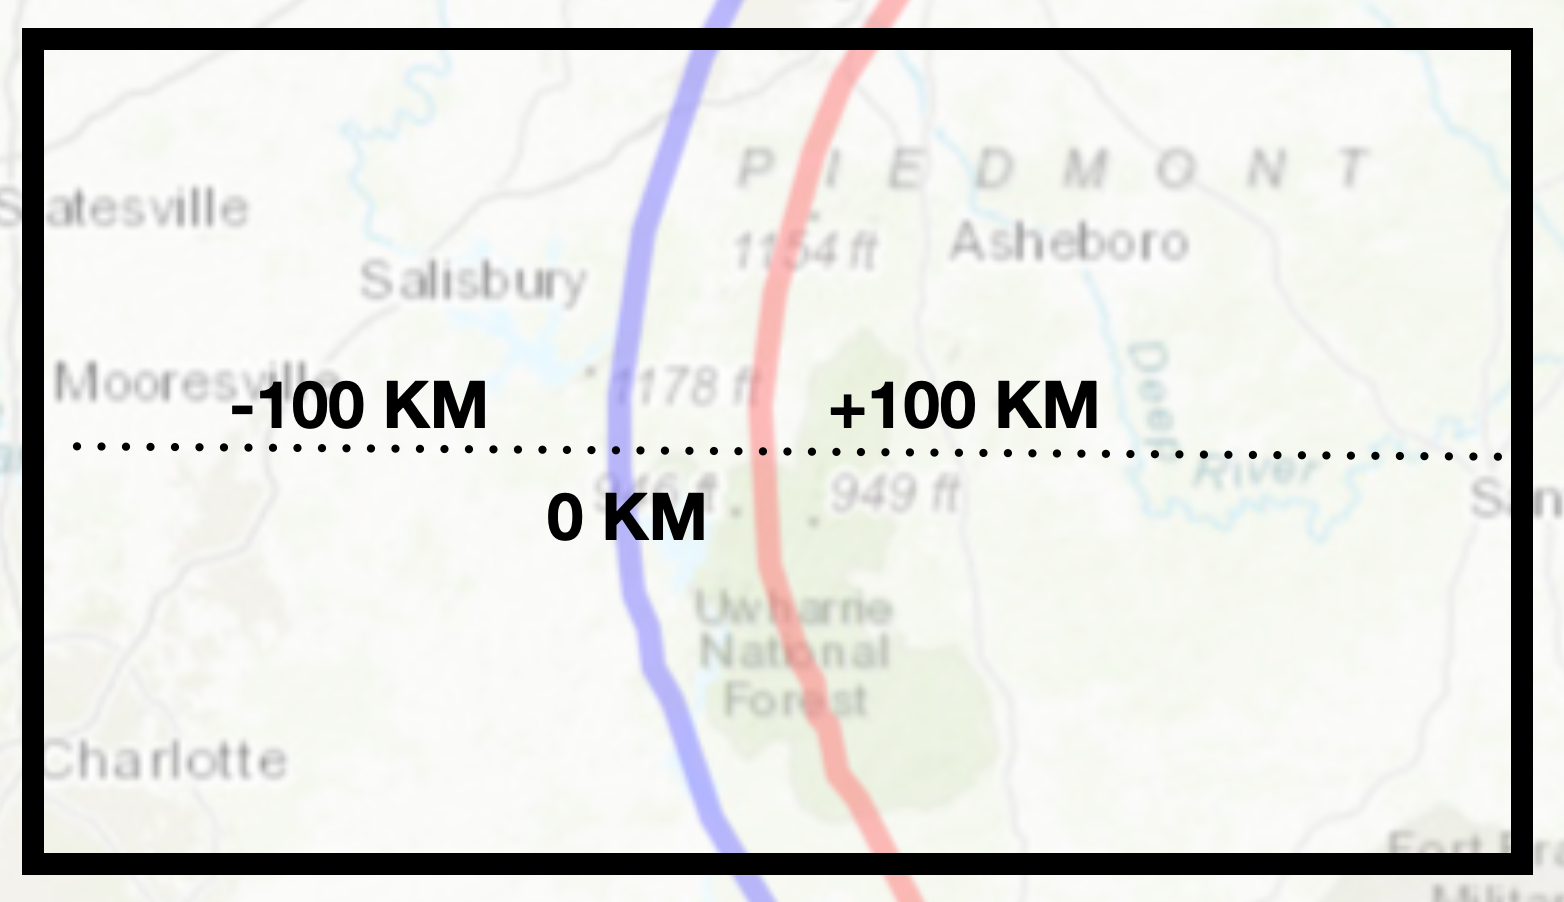
\includegraphics[width=.24\textwidth]{figs/contour_describer}\\
\end{center}
\vspace{-5pt}
\footnotesize Negative distances are outside coverage contour (no SLTV). \hyperlink{atus_breakdown}{\beamergotobutton{Time breakdown}}

%\begin{center}
%\scalebox{.8}{
%	\begin{threeparttable}
%			\begin{tabular}{lcccccccccc}
%				\hline\hline\addlinespace
%				Panel A: Minutes of TV watched &  (1) & (2) & (3) & (4) \\
%                                \hline\addlinespace
% TV Dummy $\times$ Hispanic  & 13.610$^{***}$ & 14.638$^{***}$ & 8.777$^{**}$ & 7.911$^{**}$ \\ 
%  & (3.825) & (3.831) & (3.834) & (3.829) \\ 
% TV Dummy & $-$1.170 & $-$1.392 & 4.096$^{**}$ & 5.030$^{**}$ \\ 
%  & (1.944) & (1.945) & (1.960) & (1.958) \\ 
%Observations & 91,315 & 91,315 & 91,315 & 91,315 \\              
%\hline\hline\addlinespace
%County \% Hispanic & No & Yes & Yes & Yes \\
%Log(Income) & No & No & Yes & Yes \\
%Person is Migrant & No & No & No & Yes \\
%				\addlinespace\hline\hline
%			\end{tabular}
%			\begin{tablenotes}[flushleft]
%				\item \textit{Notes:} 
%			\end{tablenotes}
%		\end{threeparttable}
%        }
%\end{center}
 

\end{frame}


%%%%%% SCHOOLS %%%%%%
\begin{frame}

\huge {\color{darkblue} Effect of SLTV on the Hispanic achievement gap}

\end{frame}




\begin{frame}
\frametitle{Effect of SLTV on Hispanic vs. Asian academic achievement}
\begin{center}
\scalebox{.8}{
	\begin{threeparttable}
			\begin{tabular}{lcccccccccc}
				\hline\hline\addlinespace
%				& \multicolumn{4}{c}{\textit{Minutes of TV watched}}  \\  				\cmidrule(lr){2-5} 
				&  (1) & (2) & (3)  \\
				\addlinespace\hline\addlinespace
				\multicolumn{3}{l}{Panel A: IHS(SAT/ACTs taken)} \\ %edu_dda_satactOLSIHS_spec3
                              	\hline\addlinespace
				TV dummy $\times$ Hispanic & 0.1598$^{***}$ & 0.1598$^{***}$ & 0.1598$^{***}$\\
  &(0.0264) & (0.0264) & (0.0264)\\
				\hline\hline\addlinespace
				\multicolumn{3}{l}{Panel B: IHS(calculus taken)} \\ %edu_dda_calcOLSIHS_spec3
                              	\hline\addlinespace
				 TV dummy $\times$ Hispanic & 0.2718$^{***}$ & 0.2718$^{***}$ & 0.2718$^{***}$\\
				    &(0.0369) & (0.0369) & (0.0369)\\
				\hline\hline\addlinespace
				\multicolumn{3}{l}{Panel C: IHS(APs passed)} \\ %edu_dda_appOLSIHS_spec3
                              	\hline\addlinespace
				 TV dummy $\times$ Hispanic & 0.0964$^{***}$ & 0.0966$^{***}$ & 0.0972$^{***}$\\
				  &(0.0346) & (0.0353) & (0.0360)\\
				\hline\hline\addlinespace
				\# Hispanic, Asian students & Yes & Yes  & Yes\\
                                	School size controls & No & Yes & Yes\\
                                	School type controls & No & No & Yes \\
					\addlinespace\hline\hline
			\end{tabular}
			\begin{tablenotes}[flushleft]
				\item \textit{Notes:}  School district fixed effects are always included. Standard errors are clustered at the school district level.
			\end{tablenotes}
		\end{threeparttable}
        }
\end{center}
\end{frame}

\begin{frame}
\frametitle{Effect sizes: how much is inequality reduced?}

\begin{center}
\scalebox{0.88}{

%			\begin{tabular}{lc|ccccccccc}
%				\hline\hline\addlinespace
%				& Gap vs. white & Gap vs. Asian & Gap after SLTV \\
%				\cmidrule(lr){2-2}\cmidrule(lr){3-3}\cmidrule(lr){4-4}&  (1) & (2) & (3)  \\
%				\addlinespace\hline\addlinespace
%				SAT/ACTs taken & 36.6 \% & 46.8\% & 38.3\%  \\
%				Calculus taken & 15.0\% & 53.6\% & 41.0\%  \\
%				APs passed & 17.8\% & 72.3\% & 69.6\%  \\
%				Gifted students & 56.6\% & 60.5\% & 51.0\%  \\
%				Advanced math taken & 25.8\% & 45.3\% & 31.7\%  \\
%				Biology taken  & -6.2\% & 5.6\% & -18.9\% \\
%				Physics taken & 25.4\% & 43.7\% & 26.2\%  \\
%				Chemistry taken & 9.9\%  & 27.7\% & 6.7\% \\
%					\addlinespace\hline\hline
%			\end{tabular}
			\begin{tabular}{lc|ccccccccc}
				\hline\hline\addlinespace
				& Gap vs. Asian & Gap after SLTV \\
				\cmidrule(lr){2-2}\cmidrule(lr){3-3} &  (1) & (2)  \\
				\addlinespace\hline\addlinespace
				SAT/ACTs taken & 46.8\% & 38.3\%  \\
				Calculus taken  & 53.6\% & 41.0\%  \\
				APs passed  & 72.3\% & 69.6\%  \\
				Gifted students & 60.5\% & 51.0\%  \\
				Advanced math taken & 45.3\% & 31.7\%  \\
				Biology taken & 5.6\% & -18.9\% \\
				Physics taken & 43.7\% & 26.2\%  \\
				Chemistry taken  & 27.7\% & 6.7\% \\
					\addlinespace\hline\hline
			\end{tabular}
        }
\end{center}

So should we stick kids in front of a TV instead of sending them to school?
\end{frame}

%%%%%% SCHOOLS %%%%%%
\begin{frame}

\huge {\color{darkblue} Exploring the identity mechanism}

\end{frame}


\begin{frame}
\frametitle{Effect of SLTV on Hispanic vs. Asian identity outcomes}\label{mech_main}
\begin{center}
\scalebox{.8}{
	\begin{threeparttable}
			\begin{tabular}{lcccccccccc}
				\hline\hline\addlinespace
%				& \multicolumn{4}{c}{\textit{Minutes of TV watched}}  \\  				\cmidrule(lr){2-5} 
				&  (1) & (2) & (3)  \\
				\addlinespace\hline\addlinespace
				\multicolumn{3}{l}{Panel A: IHS(limited English proficiency)} \\ %edu_dda_satactOLSIHS_spec3
                              	\hline\addlinespace
				TV dummy $\times$ Hispanic & 0.3042$^{***}$ & 0.3042$^{***}$ & 0.3042$^{***}$\\
				  &(0.0379) & (0.0379) & (0.0379)\\
				\hline\hline\addlinespace
				\multicolumn{3}{l}{Panel B: IHS(bullied based on ethnicity)} \\ %edu_dda_calcOLSIHS_spec3
                              	\hline\addlinespace
				 TV dummy $\times$ Hispanic & 0.0015$^{*}$ & 0.0015$^{*}$ & 0.0015$^{*}$\\
				  &(0.0009) & (0.0009) & (0.0009)\\		 
				\hline\hline\addlinespace
				\# Hispanic, Asian students & Yes & Yes  & Yes\\
                                	School size controls & No & Yes & Yes\\
                                	School type controls & No & No & Yes \\
					\addlinespace\hline\hline
			\end{tabular}
			\begin{tablenotes}[flushleft]
				\item \textit{Notes:}  School district fixed effects are always included. Standard errors are clustered at the school district level. \hyperlink{mech_placebo}{\beamergotobutton{Disability and gender-based bullying placebo}}
			\end{tablenotes}
		\end{threeparttable}
        }
\end{center}
\end{frame}

\begin{frame}
\frametitle{The content of SLTV programs}
\begin{itemize}
  \setlength\itemsep{2em}
\item Data from archive.org's TV transcript database (2005 - 2015)
\begin{itemize}
\item Use keyword matching to code content of television programs
\item Variation at the television network level
\end{itemize}
\item Test three different mechanisms:
\vspace{0.6em}
\begin{itemize}
  \setlength\itemsep{0.6em}
\item \textbf{Identity:} 10.8\% of programs relate to Latin America (vs. sports/weather/local news translated into Spanish etc.)
\item \textbf{Education:} 15\% of programs that mention schools
\item \textbf{Role models:} 5.0\% of programs with good role models for children/adolescents (mostly telenovelas)
\end{itemize}
\end{itemize}
\end{frame}

\begin{frame}
\frametitle{Differential effect of SLTV by program content} \label{transcript_sat}
\begin{center}
\scalebox{.8}{
	\begin{threeparttable}
			\begin{tabular}{lcccccccccc}
				\hline\hline\addlinespace
%				& \multicolumn{4}{c}{\textit{Minutes of TV watched}}  \\  				\cmidrule(lr){2-5} 
				&  (1) & (2) & (3)  \\
				\addlinespace\hline\addlinespace
				\multicolumn{3}{l}{Panel A: IHS(SAT/ACTs taken)} \\ %edu_dda_satactOLSIHS_spec3
                              	\hline\addlinespace
				 TV $\times$ Hispanic $\times$ \% programs on identity & 2.313$^{**}$ &  &  \\ 
				  & (0.943) &  &  \\ 
				 TV $\times$ Hispanic $\times$ \% programs on education &  & $-$0.516 &  \\ 
				  &  & (0.626) &  \\ 
				 TV $\times$ Hispanic $\times$ \% programs with role models &  &  & $-$2.085 \\ 
				  &  &  & (2.151) \\ 
				\hline\hline\addlinespace
				\# Hispanic, Asian students & Yes & Yes  & Yes\\
                                	School size controls & No & Yes & Yes\\
                                	School type controls & No & No & Yes \\
					\addlinespace\hline\hline
			\end{tabular}
			\begin{tablenotes}[flushleft]
				\item \textit{Notes:}  School district fixed effects are always included. Standard errors are clustered at the school district level. See effect for: \hyperlink{transcript_calc}{\beamergotobutton{Calculus}} \hyperlink{transcript_ap}{\beamergotobutton{AP exams}}
			\end{tablenotes}
		\end{threeparttable}
        }
\end{center}
\end{frame}

%%% More ID
\begin{frame}
\frametitle{More on identity}\label{identity_more}
\begin{itemize}
  \setlength\itemsep{2em}
\item Hispanics \textbf{visit more Hispanic-branded establishments} (restaurants, recreation businesses) when they have access to SLTV \hyperlink{safegraph_data}{\beamergotobutton{Data and table}}
\begin{itemize}
\item However, they are no more likely to visit Brazilian establishments (or Japanese, or Cajun/Creole etc.)
\end{itemize}
\item Counties with SLTV are more \textbf{socially connected with Latin America} \hyperlink{sci_data}{\beamergotobutton{Data and table}}
\begin{itemize}
\item However, they are not more connected to Brazil (or the rest of the world)
\end{itemize}
\end{itemize}
\end{frame}

%%%%% CONTRIBUTION %%%%%%
\begin{frame}
\frametitle{Contribution}
\begin{itemize}

\item Gentzkow \& Shapiro 2008 shows how English language TV benefits students: English acquisition/cognitive channel

\item[$\rightarrow $] \textcolor{darkblue}{Provide evidence on non-cognitive, \textit{identity} based channel}


%\item Prior work on Hispanic media focused on \textit{local} political outcomes {\footnotesize (Velez \& Newman 2019; Trujillo \& al. 2012)}. 
%
%\item[$\rightarrow $] \textcolor{darkblue}{Provide a first look at how media affects Hispanic educational outcomes}

%\item[$\rightarrow $] \textcolor{darkblue}{Identify causal effect on larger scale and with more granularity (geocoded microdata)}

\pause

\item Existing research that shows identity is a powerful mechanism driving meaningful outcomes {\footnotesize (Benjamin \& al. 2007; Bursztyn \& al. 2015)}. New research on how identity is constructed and strengthened {\footnotesize (Atkin \& al. 2019; Bazzi \& al. 2019)}

\item In much of the education lit. a salient minority identity is bad because of reasons like stereotype threat {\footnotesize (Spencer, Logel, \& Davies 2016)}

\item[$\rightarrow $] \textcolor{darkblue}{Show how identity can be bolstered by the media and how it can help reduce inequality}\\ 

\end{itemize}

\end{frame}

%%%%% CONCLUSION

\begin{frame}
\frametitle{Conclusion}
\begin{itemize}
\item Hopefully persuaded you that an identity mechanism matters for Hispanic educational achievement
\begin{itemize}
\item But there could also be other important ones!
\item TV appears to be one way to operationalise the identity mechanism in schools, what are others?
\end{itemize}
\item Many ways that identity mechanism itself could operate (meta-mechanisms): 
\begin{itemize}
\footnotesize
\item Stronger ties abroad
\item Self-confidence from representation on screen
\item Stronger in-group ties within school community
\item Greater connection with parents and support network
\item Recognise relative privilege vs. countries of origin \& raise perceived value of education
\item More engagement and intellectual stimulation 
\end{itemize}

\end{itemize}
\end{frame}

		
\begin{frame}
\Large \centering \textcolor{darkblue}{Thank You!}
\end{frame}




%%%%%%% APPENDIX %%%%%%%%%%


\begin{frame}
\frametitle{TV viewership across the SLTV boundary} \label{atus_breakdown}

\begin{center}
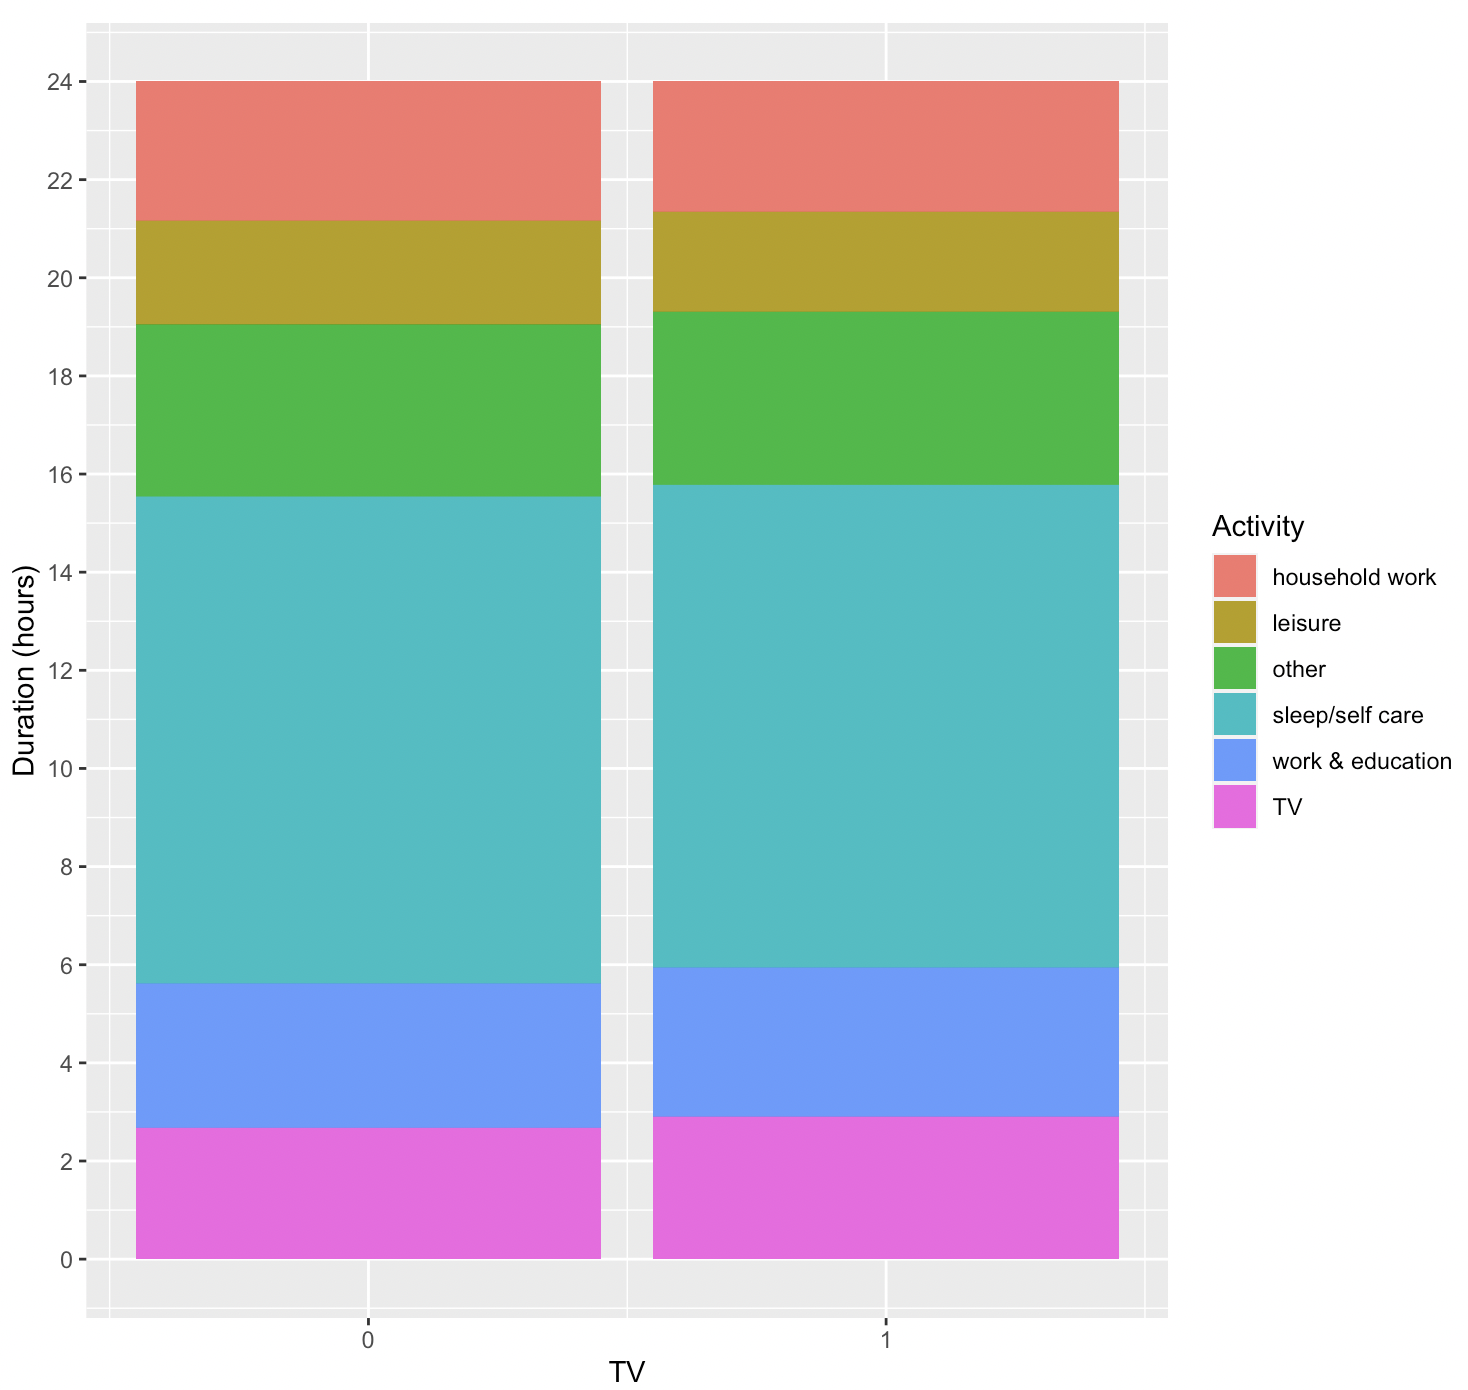
\includegraphics[width=.75\textwidth]{../../analysis/Output/graphs/time_breakdown.png}\\
\end{center}
\vspace{-5pt}
\footnotesize Hispanics with and without SLTV \hyperlink{atus_time}{\beamergotobutton{Back}}

\end{frame}




\begin{frame}
\frametitle{Differential effect of SLTV by program content} \label{transcript_calc}
\begin{center}
\scalebox{.8}{
	\begin{threeparttable}
			\begin{tabular}{lcccccccccc}
				\hline\hline\addlinespace
%				& \multicolumn{4}{c}{\textit{Minutes of TV watched}}  \\  				\cmidrule(lr){2-5} 
				&  (1) & (2) & (3)  \\
				\addlinespace\hline\addlinespace
				\multicolumn{3}{l}{Panel B: IHS(calculus taken)} \\ %edu_dda_appOLSIHS_spec3
                              	\hline\addlinespace
				 TV $\times$ Hispanic $\times$ \% programs on identity & 2.788$^{***}$ &  &  \\ 
				  & (1.034) &  &  \\ 
				 TV $\times$ Hispanic $\times$ \% programs on education &  & 0.829 &  \\ 
				  &  & (0.666) &  \\ 
				 TV $\times$ Hispanic $\times$ \% programs with role models &  &  & 1.616 \\ 
				  &  &  & (2.463) \\ 
				\hline\hline\addlinespace
				\# Hispanic, Asian students & Yes & Yes  & Yes\\
                                	School size controls & No & Yes & Yes\\
                                	School type controls & No & No & Yes \\
					\addlinespace\hline\hline
			\end{tabular}
			\begin{tablenotes}[flushleft]
				\item \textit{Notes:}  School district fixed effects are always included. Standard errors are clustered at the school district level. \hyperlink{transcript_sat}{\beamergotobutton{Back}}
			\end{tablenotes}
		\end{threeparttable}
        }
\end{center}
\end{frame}

\begin{frame}
\frametitle{Differential effect of SLTV by program content} \label{transcript_ap}
\begin{center}
\scalebox{.8}{
	\begin{threeparttable}
			\begin{tabular}{lcccccccccc}
				\hline\hline\addlinespace
%				& \multicolumn{4}{c}{\textit{Minutes of TV watched}}  \\  				\cmidrule(lr){2-5} 
				&  (1) & (2) & (3)  \\
				\addlinespace\hline\addlinespace
				\multicolumn{3}{l}{Panel C: IHS(APs passed)} \\ %edu_dda_calcOLSIHS_spec3
                              	\hline\addlinespace
				 TV $\times$ Hispanic $\times$ \% programs on identity & 1.721 &  &  \\ 
				  & (1.280) &  &  \\
				 TV $\times$ Hispanic $\times$ \% programs on education &  & 0.903 &  \\ 
				  &  & (0.922) &  \\ 
				 TV $\times$ Hispanic $\times$ \% programs with role models &  &  & $-$1.184 \\ 
				  &  &  & (2.989) \\ 
				\hline\hline\addlinespace
				\# Hispanic, Asian students & Yes & Yes  & Yes\\
                                	School size controls & No & Yes & Yes\\
                                	School type controls & No & No & Yes \\
					\addlinespace\hline\hline
			\end{tabular}
			\begin{tablenotes}[flushleft]
				\item \textit{Notes:}  School district fixed effects are always included. Standard errors are clustered at the school district level. \hyperlink{transcript_sat}{\beamergotobutton{Back}}
			\end{tablenotes}
		\end{threeparttable}
        }
\end{center}
\end{frame}

\begin{frame}
\frametitle{Effect of SLTV on foot traffic} \label{mech_placebo}
\begin{center}
\scalebox{.8}{
	\begin{threeparttable}
			\begin{tabular}{lcccccccccc}
				\hline\hline\addlinespace
%				& \multicolumn{4}{c}{\textit{Minutes of TV watched}}  \\  				\cmidrule(lr){2-5} 
				&  (1) & (2) & (3)  \\
				\addlinespace\hline\addlinespace
				\multicolumn{3}{l}{Panel A: IHS(IDEA (disability) students)} \\ %edu_dda_satactOLSIHS_spec3
                              	\hline\addlinespace
				TV dummy $\times$ Hispanic & 0.0318 & 0.0325 & 0.0318\\
  &(0.0338) & (0.0339) & (0.0338)\\
				\hline\hline\addlinespace
				\multicolumn{3}{l}{Panel B: IHS(bullied based on sex)} \\ %edu_dda_calcOLSIHS_spec3
                              	\hline\addlinespace
				TV dummy $\times$ Hispanic & 0.0090 & 0.0088 & 0.0088\\
  &(0.0056) & (0.0055) & (0.0055)\\	 
				\hline\hline\addlinespace
				\# Hispanic, Asian students & Yes & Yes  & Yes\\
                                	School size controls & No & Yes & Yes\\
                                	School type controls & No & No & Yes \\
					\addlinespace\hline\hline
			\end{tabular}
			\begin{tablenotes}[flushleft]
				\item \textit{Notes:}  School district fixed effects are always included. Standard errors are clustered at the school district level. \hyperlink{mech_main}{\beamergotobutton{Back}}
			\end{tablenotes}
		\end{threeparttable}
        }
\end{center}
\end{frame}

\begin{frame} 
\frametitle{Data: foot traffic} \label{safegraph_data}
\begin{itemize}
\item Safegraph foot traffic data in 2019 to 136,000 establishments across the US
\begin{itemize}
\item Restaurants are coded by Safegraph into different types of cuisine (11.6\% are Hispanic)
\item Other recreational establishments are manually classified using keyword matching (10.7\% are Hispanic)
\item Use census data to impute identity of visitors
\end{itemize}
\item Run regressions at the establishment-visitor demographic level to see what kind of places Hispanics are more likely to visit
\begin{itemize}
\item Main focus is on Hispanic-branded establishments
\item Three placebos: Brazilian, Japanese, and Creole/Cajun
\end{itemize}
\end{itemize}
\end{frame}

\begin{frame}
\frametitle{Effect of SLTV on foot traffic} \label{safegraph_main}
\begin{center}
\scalebox{.8}{
	\begin{threeparttable}
			\begin{tabular}{lcccccccccc}
				\hline\hline\addlinespace
				& \multicolumn{4}{c}{\textit{IHS(visitors to location)}}  \\  				
				\cmidrule(lr){2-5} &  (1) & (2) & (3) & (4) \\
				\addlinespace\hline\addlinespace
				\multicolumn{4}{l}{Panel A.1: Restaurants --- Hispanic establishment indicator} \\ 
                              	\hline\addlinespace
				TV $\times$ Hispanic $\times$ Hispanic food&       0.872***&       0.872***&       0.872***&       0.872***\\
		                  &     (0.062)   &     (0.062)   &     (0.062)   &     (0.062)   \\
				\hline\hline\addlinespace
				\multicolumn{4}{l}{Panel B.1: Recreation --- Hispanic establishment indicator} \\ 
                              	\hline\addlinespace
				TV $\times$ Hispanic $\times$ Hispanic brand&        0.569***&       0.569***&       0.569***&       0.569***\\
                    &     (0.137)   &     (0.137)   &     (0.137)   &     (0.137)   \\	
				\hline\hline\addlinespace
				County log(income) & Yes & Yes & Yes & Yes \\
				County \% Hispanic & No & Yes & Yes & Yes \\
				County log(pop.) & No & No & Yes & Yes \\
				County FE & No & No & No & Yes \\
				NAICS code FE & No & No & No & Yes \\
					\addlinespace\hline\hline
			\end{tabular}
			\begin{tablenotes}[flushleft]
				\item \textit{Notes:}  Standard errors are clustered at the county level. See placebos for: \hyperlink{safegraph_brazil}{\beamergotobutton{Brazilian}} \hyperlink{safegraph_japan}{\beamergotobutton{Japanese}}  \hyperlink{safegraph_creole}{\beamergotobutton{Creole/Cajun}} establishments. \hyperlink{identity_more}{\beamergotobutton{Back}}
			\end{tablenotes}
		\end{threeparttable}
        }
\end{center}
\end{frame}



\begin{frame}
\frametitle{Data: Social Connectedness} \label{sci_data}
\begin{itemize}
\item Facebook Social Connectedness Data from 2020
\begin{itemize}
\item County-country pairs coded by $\frac{FB Connections_{ij}}{FB Users_{i} \times FB Users_{j}}$
\item Captures relative strength of connection between US county and foreign country
\item Connectedness with other countries ranges from $0.02$ to $381$, mean value $9.388$
\end{itemize}
\end{itemize}
\end{frame}

\begin{frame}
\frametitle{Effect of SLTV on connection to Latin America} \label{sci_main}
\begin{center}
\scalebox{.8}{
	\begin{threeparttable}
			\begin{tabular}{lcccccccccc}
				\hline\hline\addlinespace
				& \multicolumn{3}{c}{\textit{SCI index}}  \\  				
				\cmidrule(lr){2-4} &  (1) & (2) & (3) \\
				\addlinespace\hline\addlinespace
				\multicolumn{4}{l}{Panel A: Latin America vs. rest of world} \\ 
                              	\hline\addlinespace
				TV dummy $\times$ Latin America & 22.023$^{***}$ & 22.023$^{***}$ & 22.023$^{***}$\\
				  &(6.837) & (6.838) & (6.839)\\
				\hline\hline\addlinespace
				\multicolumn{4}{l}{Panel B: Latin America vs. Brazil} \\ 
                              	\hline\addlinespace
				 TV dummy $\times$ Latin America & 19.703$^{***}$ & 19.703$^{***}$ & 19.703$^{***}$\\
				  &(6.219) & (6.220) & (6.221)\\
				\hline\hline\addlinespace
				County log(income) & Yes & Yes & Yes \\
				County \% Hispanic & No & Yes & Yes \\
				County log(pop.) & No & No & Yes  \\
					\addlinespace\hline\hline
			\end{tabular}
			\begin{tablenotes}[flushleft]
				\item \textit{Notes:}  Standard errors are clustered at the state level. \hyperlink{identity_more}{\beamergotobutton{Back}}
			\end{tablenotes}
		\end{threeparttable}
        }
\end{center}
\end{frame}

\begin{frame}
\frametitle{Effect of SLTV on foot traffic to Brazilian establishments} \label{safegraph_brazil}
\begin{center}
\scalebox{.8}{
	\begin{threeparttable}
			\begin{tabular}{lcccccccccc}
				\hline\hline\addlinespace
				& \multicolumn{4}{c}{\textit{IHS(visitors to location)}}  \\  				
				\cmidrule(lr){2-5} &  (1) & (2) & (3) & (4) \\
				\addlinespace\hline\addlinespace
				\multicolumn{4}{l}{Panel A.2: Restaurants --- Brazilian establishment indicator} \\ 
                              	\hline\addlinespace
				Hispanic $\times$ TV $\times$ Brazilian food&   0.058   &       0.058   &       0.058   &       0.058   \\
                    &     (0.241)   &     (0.241)   &     (0.241)   &     (0.241)   \\
				\hline\hline\addlinespace
				\multicolumn{4}{l}{Panel B.2: Recreation --- Brazilian establishment indicator} \\
                              	\hline\addlinespace
					Hispanic $\times$ TV $\times$ Brazilian brand&      0.328 & 0.328 & 0.328 & 0.328 \\
		                    &     (0.598)   &     (0.598)   &     (0.599)   &     (0.610)   \\
				\hline\hline\addlinespace
				County log(income) & Yes & Yes & Yes & Yes \\
				County \% Hispanic & No & Yes & Yes & Yes \\
				County log(pop.) & No & No & Yes & Yes \\
				County FE & No & No & No & Yes \\
				NAICS code FE & No & No & No & Yes \\
					\addlinespace\hline\hline
			\end{tabular}
			\begin{tablenotes}[flushleft]
				\item \textit{Notes:}  Standard errors are clustered at the county level. \hyperlink{safegraph_main}{\beamergotobutton{Back}}
			\end{tablenotes}
		\end{threeparttable}
        }
\end{center}
\end{frame}


\begin{frame}
\frametitle{Effect of SLTV on foot traffic to Japanese establishments} \label{safegraph_japan}
\begin{center}
\scalebox{.8}{
	\begin{threeparttable}
			\begin{tabular}{lcccccccccc}
				\hline\hline\addlinespace
				& \multicolumn{4}{c}{\textit{IHS(visitors to location)}}  \\  				
				\cmidrule(lr){2-5} &  (1) & (2) & (3) & (4) \\
				\addlinespace\hline\addlinespace
				\multicolumn{4}{l}{Panel A.3: Restaurants --- Japanese establishment indicator} \\ 
                              	\hline\addlinespace
				TV $\times$ Hispanic $\times$ Japanese food&        0.010   &       0.010   &       0.010   &       0.010   \\
                    &     (0.067)   &     (0.067)   &     (0.067)   &     (0.067)   \\
				\hline\hline\addlinespace
				\multicolumn{4}{l}{Panel B.3: Recreation --- Japanese establishment indicator} \\
                              	\hline\addlinespace
				TV $\times$ Hispanic $\times$ Japanese brand&        0.702   &       0.702   &       0.702   &       0.702   \\
                    &     (0.528)   &     (0.528)   &     (0.528)   &     (0.528)   \\
				\hline\hline\addlinespace
				County log(income) & Yes & Yes & Yes & Yes \\
				County \% Hispanic & No & Yes & Yes & Yes \\
				County log(pop.) & No & No & Yes & Yes \\
				County FE & No & No & No & Yes \\
				NAICS code FE & No & No & No & Yes \\
					\addlinespace\hline\hline
			\end{tabular}
			\begin{tablenotes}[flushleft]
				\item \textit{Notes:}  Standard errors are clustered at the county level. \hyperlink{safegraph_main}{\beamergotobutton{Back}} 
			\end{tablenotes}
		\end{threeparttable}
        }
\end{center}
\end{frame}


\begin{frame}
\frametitle{Effect of SLTV on foot traffic to Cajun/Creole establishments} \label{safegraph_creole}
\begin{center}
\scalebox{.8}{
	\begin{threeparttable}
			\begin{tabular}{lcccccccccc}
				\hline\hline\addlinespace
				& \multicolumn{4}{c}{\textit{IHS(visitors to location)}}  \\  				
				\cmidrule(lr){2-5} &  (1) & (2) & (3) & (4) \\
				\addlinespace\hline\addlinespace
				\multicolumn{4}{l}{Panel A.4: Restaurants --- Cajun and Creole establishment indicator} \\ 
                              	\hline\addlinespace
				TV $\times$ Hispanic $\times$ Cajun and Creole food&       0.174   &       0.174   &       0.174   &       0.174   \\
                    &     (0.196)   &     (0.196)   &     (0.196)   &     (0.196)   \\
				\hline\hline\addlinespace
				\multicolumn{4}{l}{Panel B.4: Recreation --- Cajun and Creole establishment indicator} \\ 
                              	\hline\addlinespace
				TV $\times$ Hispanic $\times$ Cajun and Creole brand&      -0.187 & -0.187 & -0.187 & -0.187 \\
				& (1.630)  & (1.630)& (1.630) & (1.631) \\
				\hline\hline\addlinespace
				County log(income) & Yes & Yes & Yes & Yes \\
				County \% Hispanic & No & Yes & Yes & Yes \\
				County log(pop.) & No & No & Yes & Yes \\
				County FE & No & No & No & Yes \\
				NAICS code FE & No & No & No & Yes \\
					\addlinespace\hline\hline
			\end{tabular}
			\begin{tablenotes}[flushleft]
				\item \textit{Notes:}  Standard errors are clustered at the county level. \hyperlink{safegraph_main}{\beamergotobutton{Back}} 
			\end{tablenotes}
		\end{threeparttable}
        }
\end{center}
\end{frame}



\end{document}


























